\documentclass[11pt, a4paper]{article}\usepackage[]{graphicx}\usepackage[]{xcolor}
% maxwidth is the original width if it is less than linewidth
% otherwise use linewidth (to make sure the graphics do not exceed the margin)
\makeatletter
\def\maxwidth{ %
  \ifdim\Gin@nat@width>\linewidth
    \linewidth
  \else
    \Gin@nat@width
  \fi
}
\makeatother

\definecolor{fgcolor}{rgb}{0.345, 0.345, 0.345}
\newcommand{\hlnum}[1]{\textcolor[rgb]{0.686,0.059,0.569}{#1}}%
\newcommand{\hlsng}[1]{\textcolor[rgb]{0.192,0.494,0.8}{#1}}%
\newcommand{\hlcom}[1]{\textcolor[rgb]{0.678,0.584,0.686}{\textit{#1}}}%
\newcommand{\hlopt}[1]{\textcolor[rgb]{0,0,0}{#1}}%
\newcommand{\hldef}[1]{\textcolor[rgb]{0.345,0.345,0.345}{#1}}%
\newcommand{\hlkwa}[1]{\textcolor[rgb]{0.161,0.373,0.58}{\textbf{#1}}}%
\newcommand{\hlkwb}[1]{\textcolor[rgb]{0.69,0.353,0.396}{#1}}%
\newcommand{\hlkwc}[1]{\textcolor[rgb]{0.333,0.667,0.333}{#1}}%
\newcommand{\hlkwd}[1]{\textcolor[rgb]{0.737,0.353,0.396}{\textbf{#1}}}%
\let\hlipl\hlkwb

\usepackage{framed}
\makeatletter
\newenvironment{kframe}{%
 \def\at@end@of@kframe{}%
 \ifinner\ifhmode%
  \def\at@end@of@kframe{\end{minipage}}%
  \begin{minipage}{\columnwidth}%
 \fi\fi%
 \def\FrameCommand##1{\hskip\@totalleftmargin \hskip-\fboxsep
 \colorbox{shadecolor}{##1}\hskip-\fboxsep
     % There is no \\@totalrightmargin, so:
     \hskip-\linewidth \hskip-\@totalleftmargin \hskip\columnwidth}%
 \MakeFramed {\advance\hsize-\width
   \@totalleftmargin\z@ \linewidth\hsize
   \@setminipage}}%
 {\par\unskip\endMakeFramed%
 \at@end@of@kframe}
\makeatother

\definecolor{shadecolor}{rgb}{.97, .97, .97}
\definecolor{messagecolor}{rgb}{0, 0, 0}
\definecolor{warningcolor}{rgb}{1, 0, 1}
\definecolor{errorcolor}{rgb}{1, 0, 0}
\newenvironment{knitrout}{}{} % an empty environment to be redefined in TeX

\usepackage{alltt}

\usepackage[top = 0.6 in, bottom = 0.6 in, left = 0.8 in, right = 0.8 in]{geometry}
\usepackage{amsmath, amssymb, amsfonts}

\allowdisplaybreaks[4]

\usepackage{enumerate}
\usepackage{array}
\usepackage{multirow}
\usepackage{dingbat}
\usepackage{fontawesome5}
\usepackage{tasks}
\usepackage{bbding}
\usepackage{twemojis}
% how to use bull's eye ----- \scalebox{2.0}{\twemoji{bullseye}}
\usepackage{fontspec}
\usepackage{fancyhdr}
\usepackage{lastpage}

\pagestyle{fancy}
\fancyhf{}
\fancyfoot[C]{Page \thepage\ of \pageref{LastPage}}
\renewcommand{\headrulewidth}{0pt}

\title{Bootstrapping Technique}
\author{{\fontsize{22}{20} \benyorithafont Ananda Biswas}}
\date{}

\newfontface\benyorithafont{Benyoritha-G334D.otf}

\newfontface\myfont{Myfont1-Regular.ttf}[LetterSpace=0.05em]

\newfontface\gloriahallelujahfont{GLORIAHALLELUJAH-REGULAR.TTF}

\newfontface\cbfont{CaveatBrush-Regular.ttf}
% how to use --- \myfont --write text here--
\IfFileExists{upquote.sty}{\usepackage{upquote}}{}
\begin{document}

\maketitle


\section*{\faArrowAltCircleRight[regular] \textcolor{blue}{Introduction}}

Bootstrapping is a resampling technique used to approximate the sampling distribution of a statistic when the true distribution is unknown or hard to derive analytically. Instead of generating new samples from population, we take repeated with-replacement samples from the observed sample. This creates many new samples, called \textbf{bootstrap samples} that mimic resampling from the population.

\begin{enumerate}[Step I.]
\item Obtain sample $x_1, x_2, \ldots, x_n$. Based on this sample, let $\hat{\theta}$ be an estimator of population parameter $\theta$. Treat this sample as empirical population.

\item Draw bootstrap sample of size $n$ with-replacement from $\{x_1, x_2, \ldots, x_n\}$.

\item Compute the estimate $\widehat{\theta_{j}^{*}}$ for the drawn bootstrap sample.

\item Repeat steps II and III both $B$ times to obtain $$\widehat{\theta_{1}^{*}}, \widehat{\theta_{2}^{*}}, \ldots, \widehat{\theta_{B}^{*}}.$$
\end{enumerate}

$\{\widehat{\theta_{1}^{*}}, \widehat{\theta_{2}^{*}}, \ldots, \widehat{\theta_{B}^{*}}\}$ can be treated as a sample from the sampling distribution of $\hat{\theta}$ and can be used for further inferences \textit{e.g.} estimating the variability of an estimator. \\[0.3em]

$\bullet$ \textbf{Bootstrap estimate of Bias, Standard Error \& MSE} of $\hat{\theta}$ are given by $$\text{Bias}_{\text{boot}} = \dfrac{1}{B} \sum \limits_{b = 1}^{B} \widehat{\theta_{b}^{*}} - \hat{\theta} \qquad \& \qquad \text{SE}_{\text{boot}} = \sqrt{\dfrac{1}{B-1} \sum \limits_{b = 1}^{B} \left[\widehat{\theta_{b}^{*}} - \overline{\theta^*}\right]^2} \qquad \& \qquad \text{MSE}_{\text{boot}} = \dfrac{1}{B} \sum \limits_{b = 1}^{B} \left[\widehat{\theta_{b}^{*}} - \hat{\theta}\right]^2$$

\begin{align*}
\text{where } \hat{\theta} &: \text{ estimate of } \theta \text{ from the original sample}, \\[0.2em]
\widehat{\theta_{b}^{*}} &: \text{ estimate of } \theta \text{ from } b\text{-th bootstrap sample}, \\[0.2em]
\overline{\theta^*} &: \text{ average of the bootstrap estimates}, \\[0.2em]
B &: \text{number of bootstrap samples drawn}.
\end{align*}

Let us have an R demo.





\begin{knitrout}
\definecolor{shadecolor}{rgb}{0.969, 0.969, 0.969}\color{fgcolor}\begin{kframe}
\begin{alltt}
\hldef{n} \hlkwb{<-} \hlnum{100}\hldef{; B} \hlkwb{<-} \hlnum{1000}\hldef{; theta} \hlkwb{<-} \hlnum{2}

\hldef{x} \hlkwb{<-} \hlkwd{rexp}\hldef{(n,} \hlkwc{rate} \hldef{= theta)}

\hldef{theta_hat} \hlkwb{<-} \hlnum{1} \hlopt{/} \hlkwd{mean}\hldef{(x); theta_hat}
\end{alltt}
\begin{verbatim}
## [1] 2.116519
\end{verbatim}
\end{kframe}
\end{knitrout}

\begin{knitrout}
\definecolor{shadecolor}{rgb}{0.969, 0.969, 0.969}\color{fgcolor}\begin{kframe}
\begin{alltt}
\hldef{bootstrap.theta_hat} \hlkwb{<-} \hlkwd{c}\hldef{()}

\hlkwa{for} \hldef{(i} \hlkwa{in} \hlnum{1}\hlopt{:}\hldef{B) \{}
  \hldef{bootstrap.sample} \hlkwb{<-} \hlkwd{sample}\hldef{(x,} \hlkwc{size} \hldef{= n,} \hlkwc{replace} \hldef{=} \hlnum{TRUE}\hldef{)}

  \hldef{bootstrap.theta_hat[i]} \hlkwb{<-} \hlnum{1} \hlopt{/} \hlkwd{mean}\hldef{(bootstrap.sample)}
\hldef{\}}

\hlkwd{head}\hldef{(bootstrap.theta_hat)}
\end{alltt}
\begin{verbatim}
## [1] 2.233834 2.142502 2.025614 2.341397 2.287169 2.234499
\end{verbatim}
\end{kframe}
\end{knitrout}




\begin{knitrout}
\definecolor{shadecolor}{rgb}{0.969, 0.969, 0.969}\color{fgcolor}
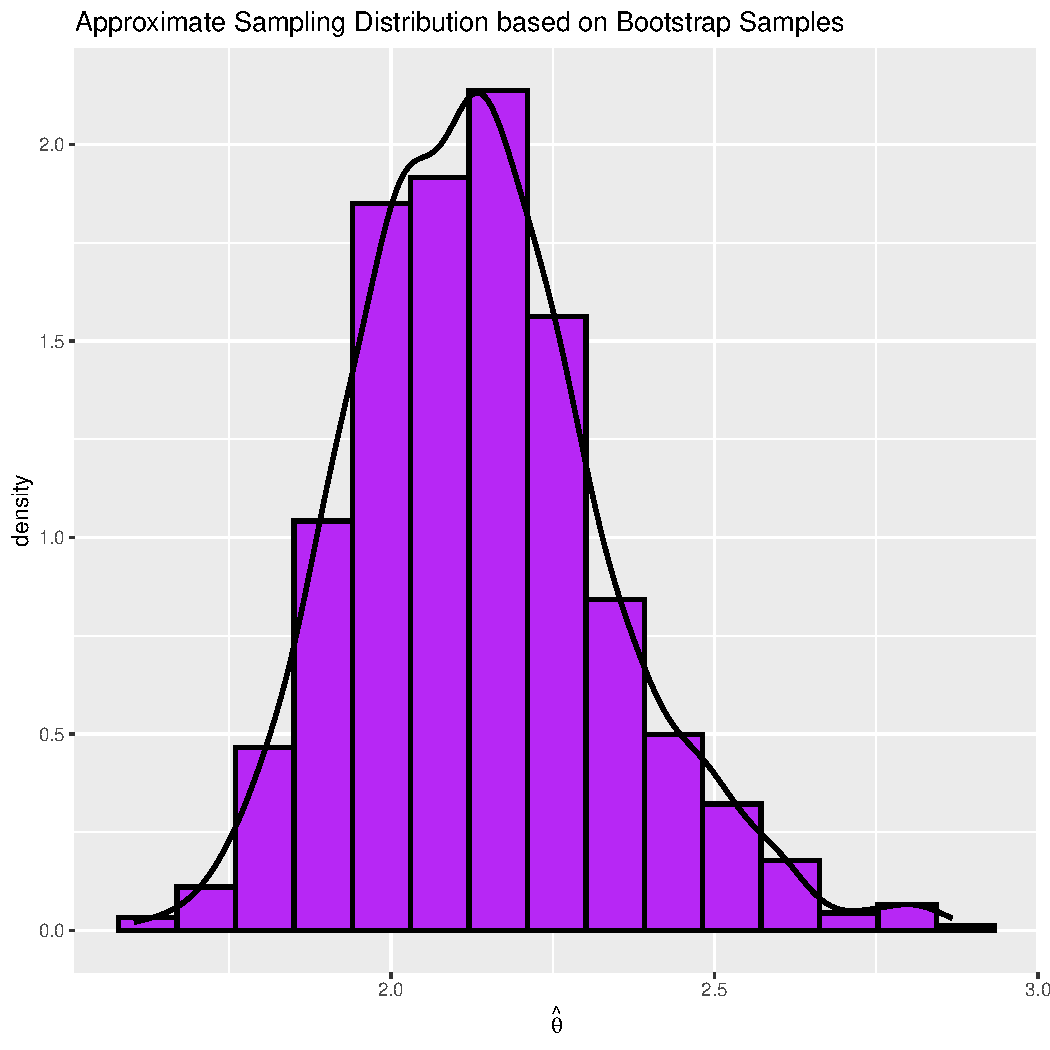
\includegraphics[width=\maxwidth]{figure/unnamed-chunk-6-1} 
\end{knitrout}

\begin{knitrout}
\definecolor{shadecolor}{rgb}{0.969, 0.969, 0.969}\color{fgcolor}\begin{kframe}
\begin{alltt}
\hldef{bootstrap.bias} \hlkwb{<-} \hlkwd{mean}\hldef{(bootstrap.theta_hat)} \hlopt{-} \hldef{theta_hat; bootstrap.bias}
\end{alltt}
\begin{verbatim}
## [1] 0.02134709
\end{verbatim}
\end{kframe}
\end{knitrout}

\begin{knitrout}
\definecolor{shadecolor}{rgb}{0.969, 0.969, 0.969}\color{fgcolor}\begin{kframe}
\begin{alltt}
\hldef{bootstrap.MSE} \hlkwb{<-} \hlkwd{mean}\hldef{((bootstrap.theta_hat} \hlopt{-} \hldef{theta_hat)}\hlopt{^}\hlnum{2}\hldef{); bootstrap.MSE}
\end{alltt}
\begin{verbatim}
## [1] 0.03901209
\end{verbatim}
\end{kframe}
\end{knitrout}

\section*{\faArrowAltCircleRight[regular] \textcolor{blue}{Bootstrap Confidence Interval}}

Using bootstrap samples, we can also construct confidence interval for $\theta$.\\[0.2em]

Recall that bootstrap estimates $\widehat{\theta_{1}^{*}}, \widehat{\theta_{2}^{*}}, \ldots, \widehat{\theta_{B}^{*}}$ approximate the sampling distribution of $\hat{\theta}$. 

\begin{enumerate}[Step I.]
\item Arrange bootstrap estimates in ascending order as $$\widehat{\theta}^{*}_{\!(1)} \leq  \widehat{\theta}^{*}_{\!(2)} \leq \ldots \leq \widehat{\theta}^{*}_{\!(B)}.$$

\item $100(1 - \alpha)\%$ confidence interval is given by $$\left( \widehat{\theta}^{*}_{\!(\alpha B / 2)}, \widehat{\theta}^{*}_{\!((1 - \alpha / 2) B)} \right).$$
\end{enumerate}

\begin{knitrout}
\definecolor{shadecolor}{rgb}{0.969, 0.969, 0.969}\color{fgcolor}\begin{kframe}
\begin{alltt}
\hlkwd{quantile}\hldef{(bootstrap.theta_hat,} \hlkwd{c}\hldef{(}\hlnum{0.025}\hldef{,} \hlnum{0.975}\hldef{))} \hlcom{# alpha = 0.05}
\end{alltt}
\begin{verbatim}
##     2.5%    97.5% 
## 1.801481 2.575581
\end{verbatim}
\end{kframe}
\end{knitrout}


So far what we have discussed is \textbf{non-parametric bootstrapping} where population distribution was not known. Another scenario called \textbf{parametric bootstrapping} is where the population distribution family is known, but the member is unknown. There we proceed as follows.

\begin{enumerate}[Step I.]
\item Suppose we have $x_1, x_2, \ldots, x_n \sim F(x, \theta)$ where functional form of $F$ is known but $\theta$ is unknown.

\item Obtain an estimate of $\theta$ as $\hat{\theta}$.

\item Plug in $\hat{\theta}$ in place of $\theta$ and generate a sample of size $n$ as $x_1^*, x_2^*, \ldots, x_n^* \sim F(x, \hat{\theta})$.

\item Based on bootstrapped sample $\{x_1^*, x_2^*, \ldots, x_n^*\}$, calculate $\widehat{\theta_{j}^{*}}$.

\item Repeat steps III and IV both $B$ times to get $$\widehat{\theta_{1}^{*}}, \widehat{\theta_{2}^{*}}, \ldots, \widehat{\theta_{B}^{*}}.$$
\end{enumerate}

$\{\widehat{\theta_{1}^{*}}, \widehat{\theta_{2}^{*}}, \ldots, \widehat{\theta_{B}^{*}}\}$ can be thought as sample from the sampling distribution of $\hat{\theta}$ and can be used to obtain bootstrap estimate of bias, MSE, confidence interval as discussed previously. \\[0.3em]

Let us have an R demo of the above.



\begin{knitrout}
\definecolor{shadecolor}{rgb}{0.969, 0.969, 0.969}\color{fgcolor}\begin{kframe}
\begin{alltt}
\hlkwd{set.seed}\hldef{(}\hlnum{14}\hldef{)}
\end{alltt}
\end{kframe}
\end{knitrout}

\begin{knitrout}
\definecolor{shadecolor}{rgb}{0.969, 0.969, 0.969}\color{fgcolor}\begin{kframe}
\begin{alltt}
\hldef{n} \hlkwb{<-} \hlnum{100}\hldef{; B} \hlkwb{<-} \hlnum{1000}\hldef{; theta} \hlkwb{<-} \hlnum{5}

\hldef{x} \hlkwb{<-} \hlkwd{rnorm}\hldef{(n,} \hlkwc{mean} \hldef{= theta,} \hlkwc{sd} \hldef{=} \hlnum{1}\hldef{)}

\hldef{theta_hat} \hlkwb{<-} \hlkwd{mean}\hldef{(x); theta_hat}
\end{alltt}
\begin{verbatim}
## [1] 5.043144
\end{verbatim}
\end{kframe}
\end{knitrout}

\begin{knitrout}
\definecolor{shadecolor}{rgb}{0.969, 0.969, 0.969}\color{fgcolor}\begin{kframe}
\begin{alltt}
\hldef{bootstrap.theta_hat} \hlkwb{<-} \hlkwd{c}\hldef{()}

\hlkwa{for}\hldef{(i} \hlkwa{in} \hlnum{1}\hlopt{:}\hldef{B)\{}
  \hldef{bootstrap.sample} \hlkwb{<-} \hlkwd{rnorm}\hldef{(n,} \hlkwc{mean} \hldef{= theta_hat,} \hlkwc{sd} \hldef{=} \hlnum{1}\hldef{)}

  \hldef{bootstrap.theta_hat[i]} \hlkwb{<-} \hlkwd{mean}\hldef{(bootstrap.sample)}
\hldef{\}}

\hlkwd{head}\hldef{(bootstrap.theta_hat)}
\end{alltt}
\begin{verbatim}
## [1] 5.040834 4.860644 5.021394 5.012305 4.947593 5.012472
\end{verbatim}
\end{kframe}
\end{knitrout}

\begin{knitrout}
\definecolor{shadecolor}{rgb}{0.969, 0.969, 0.969}\color{fgcolor}
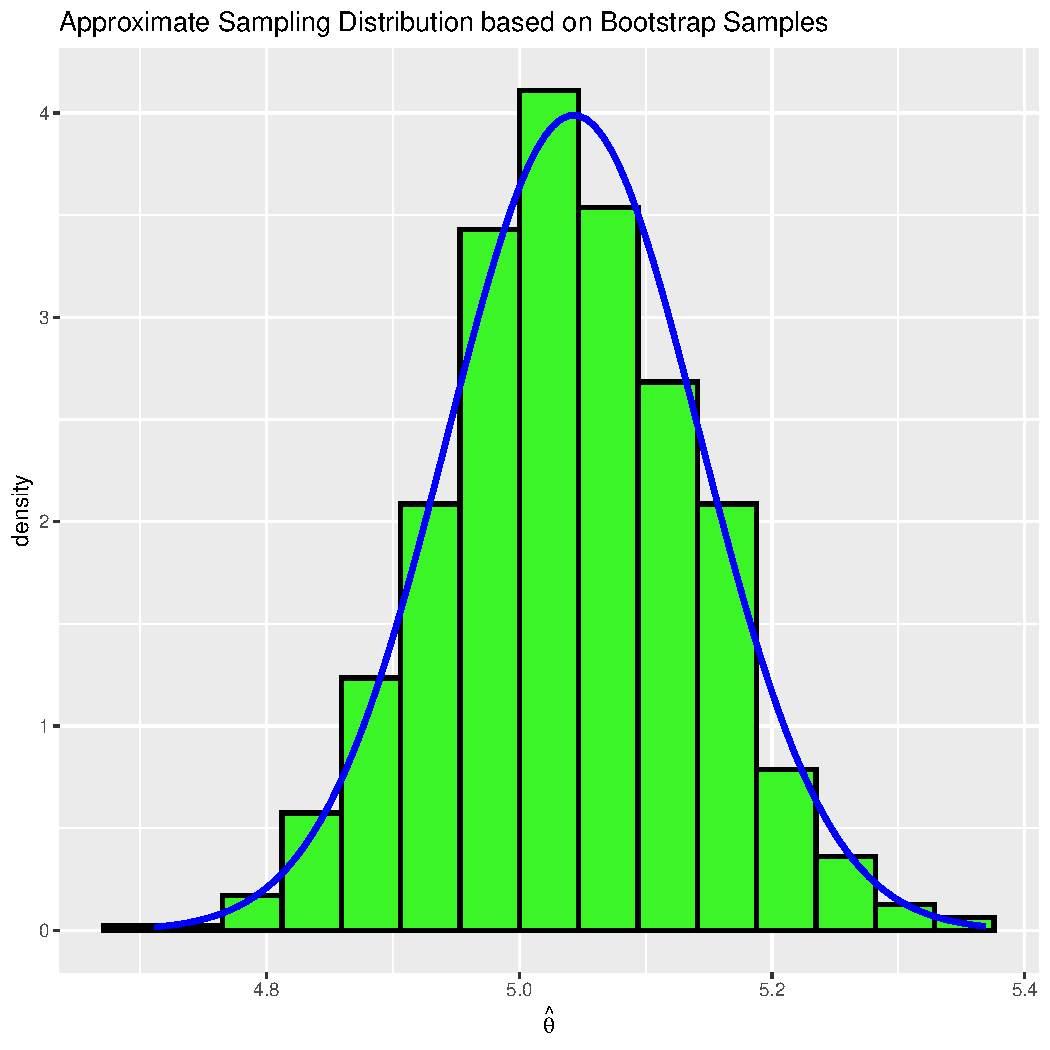
\includegraphics[width=\maxwidth]{figure/unnamed-chunk-14-1} 
\end{knitrout}

\smallpencil {\fontsize{12}{20} \gloriahallelujahfont The density in blue is of $f(x, \hat{\theta})$, it is obtained by plugging in $\hat{\theta}$ in place of $\theta$ in $f$; of course the distribution of the bootstrap estimators fits this density well.}

\end{document}
